\documentclass[10pt]{article}
\title{An Excerpt of ``The Ballot Order Effect in Taiwan's Legislative Elections, 2008--2020''}
\date{\today}

% Page layout settings
\usepackage[margin=1.5in]{geometry}
% \setlength{\parskip}{0ex plus0.5ex minus0.2ex}
\usepackage{lastpage}
\usepackage{fancyhdr}
\pagestyle{fancy}
\fancyhf{}
\renewcommand{\headrulewidth}{0pt}
\cfoot{\footnotesize Page \thepage\ of \pageref{LastPage}}
\fancypagestyle{plain}{%
  \fancyhf{}
  \renewcommand{\headrulewidth}{0pt}
  \cfoot{\footnotesize Page \thepage\ of \pageref{LastPage}}
}

\makeatletter
\def\@maketitle{%
  \noindent
  \parbox[t]{0.7\textwidth}{%
    \sffamily\bfseries\large\@title%
  }%
  \hfill
  \parbox[t]{0.3\textwidth}{%
    \raggedleft%
    \@date\\
    \@author%
  }%
  \par\vskip1.5em%
}
\makeatother

\usepackage{fontspec}
\defaultfontfeatures{Ligatures=TeX}

\usepackage{booktabs}
\usepackage{threeparttable}
\usepackage{array}

% Math packages
\usepackage{amsmath, amssymb, amsthm, accents, unicode-math}
\DeclareMathAlphabet{\mathcal}{OMS}{cmsy}{m}{n}
\let\mathbb\relax % Remove the definition by unicode-math
\DeclareMathAlphabet{\mathbb}{U}{msb}{m}{n}
\allowdisplaybreaks
% Theorem environment setup
\newtheoremstyle{sfstyle}% Name
{.5em}% Space above
{.5em}% Space below
{}% Body font
{}% Indent amount
{\bfseries\sffamily}% Theorem head font
{.}% Punctuation after theorem head
{.5em}% Space after theorem head
{}% Theorem head spec
\theoremstyle{sfstyle}
\newtheorem{theorem}{Theorem}
\newtheorem{definition}{Definition}
\newtheorem{assumption}{Assumption}
\newtheorem{remark}{Remark}
\theoremstyle{remark}
\newtheorem*{solution}{\sffamily Solution}
\renewcommand{\proofname}{\sffamily Proof}

% Section settings
% Section settings
\usepackage{titlesec}
% Section title formatting
\titleformat{\section}[hang]{\large\bfseries\sffamily}{\thesection}{1em}{}
\titleformat{\subsection}[hang]{\bfseries\sffamily}{\thesubsection}{1em}{}
\titleformat{\subsubsection}[hang]{\itshape\sffamily}{\thesubsubsection}{1em}{}
\titleformat{\paragraph}[runin]{\itshape\sffamily \color{greenblue}}{}{1em}{}
\usepackage{tocloft}
\renewcommand{\cfttoctitlefont}{\large}
\renewcommand{\contentsname}{\bfseries\sffamily Contents}
\renewcommand{\cftsecfont}{\sffamily}
\renewcommand{\cftsecpagefont}{\sffamily}
\renewcommand{\cftsubsecfont}{\sffamily}
\renewcommand{\cftsubsecpagefont}{\sffamily}

% Math operator definitions
\DeclareMathOperator{\diag}{diag}
\DeclareMathOperator{\tr}{tr}
\DeclareMathOperator{\rank}{rank}
\DeclareMathOperator{\sign}{sign}
\DeclareMathOperator*{\argmin}{argmin}
\DeclareMathOperator*{\argmax}{argmax}
\DeclareMathOperator{\supp}{supp}
\DeclareMathOperator{\Image}{Im}
\DeclareMathOperator{\Kernel}{Ker}
\DeclareMathOperator{\spn}{span}
\DeclareMathOperator{\nullity}{nullity}
\DeclareMathOperator{\E}{E}
\DeclareMathOperator{\Var}{Var}
\DeclareMathOperator{\Cov}{Cov}
\DeclareMathOperator{\ind}{\perp\!\!\!\perp}
\DeclareMathOperator{\iid}{\overset{\text{iid}}{\sim}}
\DeclareMathOperator{\cp}{\overset{\mathit{cp}}{\longrightarrow}}
\DeclareMathOperator{\as}{\overset{\mathit{a.s.}}{\longrightarrow}}
\DeclareMathOperator{\cd}{\overset{\mathit{d}}{\longrightarrow}}
\DeclareMathOperator*{\plim}{plim}

\newcommand{\bc}[1]{{\left\lbrace #1 \right\rbrace}}
\newcommand{\bp}[1]{{\left( #1 \right)}}
\newcommand{\bs}[1]{{\left[ #1 \right]}}
\newcommand{\abs}[1]{{\left| #1 \right|}}
\newcommand{\norm}[1]{{\left\| #1 \right\|}}
\newcommand{\innerproduct}[2]{{\left\langle #1, #2 \right\rangle}}

\usepackage{pgf,tikz}
\usetikzlibrary{arrows,shapes.arrows,shapes.geometric,shapes.multipart,
decorations.pathmorphing,positioning}
\tikzset{
  every picture/.style={thick},
  ell/.style={draw,fill=white,shape=ellipse,inner sep=1pt},
  cir/.style={draw,fill=white,shape=circle,inner sep=2pt},
}

\usepackage{caption}
\usepackage{subcaption}
\captionsetup{font=small}

\usepackage{enumitem}
\setlist{noitemsep}

% Bibliography packages
\usepackage{natbib}
\renewcommand{\bibfont}{\footnotesize}


% Color palette
\usepackage{xcolor}
\definecolor{greenblue}{RGB}{35, 100, 170}
\definecolor{asparagus}{RGB}{107, 170, 117}
\definecolor{darkred}{RGB}{170, 38, 35}
\definecolor{gray75}{gray}{0.75}

\usepackage{hyperref}
\hypersetup{
  colorlinks=true,
  linkcolor=greenblue,
  urlcolor=greenblue,
  citecolor=asparagus
}

\usepackage[nogroupskip,style=super,acronym]{glossaries}
\makeglossaries
\newacronym{smd}{SMD}{single-member district}
\newacronym{fptp}{FPTP}{first-past-the-post}
\newacronym{cec}{CEC}{Central Election Commission}
\newacronym{sre}{SRE}{stratified randomized experiment}
\newacronym{ate}{ATE}{average treatment effect}
\newacronym{ci}{CI}{confidence interval}
\newacronym{sutva}{SUTVA}{stable unit treatment value assumption}
\newacronym{ipw}{IPW}{inverse probability weighting}
\newacronym{dgp}{DGP}{data-generating process}
\newacronym{frt}{FRT}{Fisher randomization test}
\newacronym{ols}{OLS}{ordinary least squares}
\newacronym{fe}{FE}{fixed effects}
\newacronym{ehw}{EHW}{Eicker-Huber-White}

\glsdisablehyper

\usepackage{cleveref}
\crefname{section}{Section}{Sections}
\crefname{equation}{Equation}{Equations}
\crefname{figure}{Figure}{Figures}
\crefname{table}{Table}{Tables}

\renewcommand{\abstractname}{\sffamily\bfseries Abstract}

% CJK packages and settings
\usepackage{xeCJK}
\usepackage{fontspec}
\XeTeXlinebreaklocale "zh"
\setCJKmainfont{Songti TC}
\setCJKsansfont{Taipei Sans TC Beta}
\newCJKfontfamily\kai{Kaiti TC}

\begin{document}
\maketitle

\setcounter{section}{1}

\section{Context and Data} \label{sec:context-data}

\subsection{Institutional Context}

Since 2008, 
Taiwan's Legislative Yuan elections 
have operated under a mixed-member majoritarian system. 
This study focuses on the 73 \glspl{smd},
where legislators are elected via a \gls{fptp} system. 
According to Article 34 of the Civil Servants Election and Recall Act, 
the ballot order for candidates in each district 
is determined by a public lottery held by the electoral commission.
This procedure creates a natural experiment within each electoral district. 
Unlike the vertical ballots common in many Western countries, 
Taiwan's ballots are arranged horizontally, 
with candidates listed from left to right.

\subsection{Data}

Our data come from the official legislative election results
published by the \gls{cec} of Taiwan.
The dataset contains detailed information
for each candidate in every district from 2008 to 2020,
including electoral district,
ballot number, party affiliation, 
vote share, and incumbency status.
Our treatment variable is whether a candidate is listed first on the ballot,
and our outcome variable is the candidate's vote share.

\section{Empirical Strategies}

\subsection{Notation and Setup}

Let the index $k \in \{1, \ldots, K\}$ denote an electoral district, 
where $K=73$ for each election year. 
Within each district $k$, 
there are $n_{[k]}$ candidates,
indexed by $i \in \{1, \ldots, n_{[k]}\}$. 
For each candidate $i$ in district $k$, 
we define a binary treatment indicator, $D_{[k]i}$, 
which equals $1$ if the candidate is listed first on the ballot 
and $0$ otherwise. 
The main outcome of interest is the candidate's vote share, 
denoted by $Y_{[k]i}$.

A naive approach would be to compare 
the average vote share of all candidates listed first 
with that of all candidates not listed first:
\begin{align}
\hat{\tau}_{\text{naive}}
= \frac{1}{n_1} \sum_{k=1}^K \sum_{i: D_{[k]i} = 1} Y_{[k]i}
 - \frac{1}{n_0} \sum_{k=1}^K \sum_{i: D_{[k]i} = 0} Y_{[k]i},
 \label{eq:naive-estimator}
\end{align}
where $n_1$ and $n_0$ are the total counts of treated and control candidates, respectively.
This estimator,
however,
is biased because the number of candidates $n_{[k]}$
is a confounder that
affects both the treatment assignment probability
and the vote share distribution.

\subsection{Conventional Approaches and Their Limitations}

Two conventional methods address the confounding caused by district size.
The first approach includes \glspl{fe}
for the number of candidates in a linear regression model:
\begin{align}
  Y_{[k]i} = \alpha + \beta_{\text{fe}} D_{[k]i} +
  \sum_{s=3}^{S} \gamma_s \mathbf{1}(n_{[k]} = s) + \varepsilon_{[k]i},
  \label{eq:fixed-effects-model}
\end{align}
where districts with two candidates serve as the baseline reference group.\footnote{
  The estimator $\hat{\beta}_{\text{fe}}$ is a variance-weighted average of the
  difference-in-means estimators from each stratum, 
  giving more influence to strata 
  with larger variance in the treatment indicator.
}

The second approach relies on \gls{ipw},
which creates a pseudo-population
where the treatment assignment is independent of district size
\citep{horvitz1952generalization, hernan2020causal}.
It is convenient to implement \gls{ipw}
using a weighted linear regression model:
\begin{align}
  Y_{[k]i} = \alpha + \beta_{\text{ipw}} D_{[k]i} + \varepsilon_{[k]i},
  \label{eq:ipw-model}
\end{align}
where each observation is weighted by the inverse of its treatment assignment probability:
$$
w_{[k]i} = D_{[k]i} n_{[k]} + (1 - D_{[k]i}) \frac{n_{[k]}}{n_{[k]} - 1}.
$$

While both approaches adjust for district size confounding,
their causal interpretation requires the \gls{sutva}
\citep{cox1958planning, rubin1980discussion}.
In our context,
this assumption is likely violated
since candidates within the same district
compete for the same pool of votes,
and vote shares must sum to $100\%$.
When interference is present,
the coefficients lose their interpretation
as an \gls{ate},
and conventional standard error estimates
become invalid.
These limitations motivate us to seek
a design-based inference approach,
which leverages the known randomization mechanism
and does not rely on \gls{sutva}.

\subsection{Fisher Randomization Test}

Instead of relying on model-based inference
and questionable stability assumptions,
we can exploit the known randomization mechanism
to draw causal inferences via \gls{frt} \citep{fisher1935design}.
We conceptualize the ballot order assignment process,
as a \gls{sre},
where each electoral district constitutes a stratum.
Within each district $k$,
one candidate is randomly assigned,
to treatment (listed first),
and the remaining $n_{[k]}-1$,
candidates are assigned to control.

To formally define the \gls{frt} in our context,
we first introduce the potential outcomes framework 
\citep{neyman1923application, rubin1974estimating, rosenbaum2007interference, imbens2015causal}.
Let $\mathbf{D}_{[k]} = (D_{[k]1}, \ldots, D_{[k]n_{[k]}})$,
be a random vector representing the treatment assignments,
for all $n_{[k]}$ candidates in district $k$,
and let $\mathbf{d}_{[k]}$ be a specific realization of $\mathbf{D}_{[k]}$.
The entire set of possible ballot assignments,
for district $k$ is denoted by $\mathcal{D}_{[k]}$,
defined as
\begin{align}
  \mathcal{D}_{[k]} = \bc{\mathbf{d}_{[k]} \in \{0,1\}^{n_{[k]}} : \sum_{i=1}^{n_{[k]}} d_{[k]i} = 1}.
\end{align}
We denote the set of all possible assignments,
across all districts by $\mathcal{D} = \mathcal{D}_{[1]} \times \cdots \times \mathcal{D}_{[K]}$.
We define the potential outcome, $Y_{[k]i}(\mathbf{d}_{[k]})$,
as the vote share that candidate $i$ in district $k$ would receive,
if the ballot assignment were $\mathbf{d}_{[k]}$.
This notation explicitly allows a candidate's vote share,
to depend on which of their opponents received the treatment.
These potential outcomes are constrained,
by the institutional fact that vote shares must sum to one within a district:
\[
\sum_{i=1}^{n_{[k]}} Y_{[k]i}(\mathbf{d}_{[k]}) = 1
\]
for any valid assignment $\mathbf{d}_{[k]}$.
Notice that the potential outcomes,
are treated as fixed quantities,
and the only source of randomness,
comes from the random assignment of treatments.
The observed outcome for candidate $i$ in district $k$ is then,
$Y_{[k]i} = Y_{[k]i}(\mathbf{D}_{[k]})$.

The \gls{frt} tests the null hypothesis:
\begin{align}
  H_0:
  \;
  Y_{[k]i}(\mathbf{d}_{[k]}) = Y_{[k]i}(\mathbf{d}'_{[k]}),
  \quad \forall k,\; i,\; \mathbf{d}_{[k]},\; \mathbf{d}'_{[k]} \in \mathcal{D}_{[k]},
  \label{eq:null-hypothesis}
\end{align}
which states that
the ballot order has no effect
(neither directly nor indirectly through interference)
on any candidate's vote share.
Under $H_0$,
the \gls{sutva} automatically holds
because for each candidate,
all potential outcomes are identical.

To conduct the \gls{frt},
we must choose a test statistic
$T(\mathbf{D}, \mathbf{Y})$ a priori,
where $\mathbf{D}$ and $\mathbf{Y}$
are treatment assignment and outcome vectors
across all districts and candidates.
For simplicity,
we consider the weighted difference-in-means statistic:
\[
  T(\mathbf{D}, \mathbf{Y}) =
  \sum_{k=1}^K w_{[k]} \tau_{[k]},
\]
where $\tau_{[k]}$ is the difference-in-means estimator
within district $k$,
and the weight
\[
  w_{[k]} 
  = \frac{\frac{n_{[k]}}{n} \cdot \frac{1}{n_{[k]}} \cdot \frac{n_{[k]} - 1}{n_{[k]}}}{\sum_{k'=1}^K \frac{n_{[k']}}{n} \cdot \frac{1}{n_{[k']}} \cdot \frac{n_{[k']} - 1}{n_{[k']}}}
  = \frac{n_{[k]} - 1}{\sum_{k'=1}^K (n_{[k']} - 1)}
\]
is a weight proportional to the variance of the treatment indicator
in district $k$,
which gives more influence to larger districts
to improve efficiency.

Under \gls{sre},
the randomization distribution of $T(\mathbf{D}, \mathbf{Y})$
is uniform over $\mathcal{D}$.
Since under $H_0$ the observed outcomes $\mathbf{Y}$ are fixed,
we can simulate the null distribution of $T$
by repeatedly drawing treatment assignments from $\mathcal{D}$
and computing the corresponding test statistic.
The $p$-value,
calculated as the proportion of simulated test statistics
at least as extreme as the observed value,
quantifies how surprising the observed data are under the null hypothesis.
Given that $\mathcal{D}$ contains approximately $10^{52}$ possible assignments,
we approximate the randomization distribution via Monte Carlo simulation
with $10000$ random draws.
We also report the standard error of the $p$-value estimate
to quantify the Monte Carlo approximation error.

\section{Main Results} \label{sec:main-results}

\subsection{Conventional Estimates}

\cref{fig:effect-plot} shows 
estimated ballot order effects using 
naive comparison, fixed effects, 
and \gls{ipw} approaches. 
Among the four election years,
2016 shows the largest estimated effect.
While naive estimates suggest substantial effects 
these disappear once we control for district size, 
yielding point estimates near zero with 
no statistical significance. 
However, these conventional methods 
rely on the questionable \gls{sutva} assumption.

\begin{figure}[htbp]
  \centering
  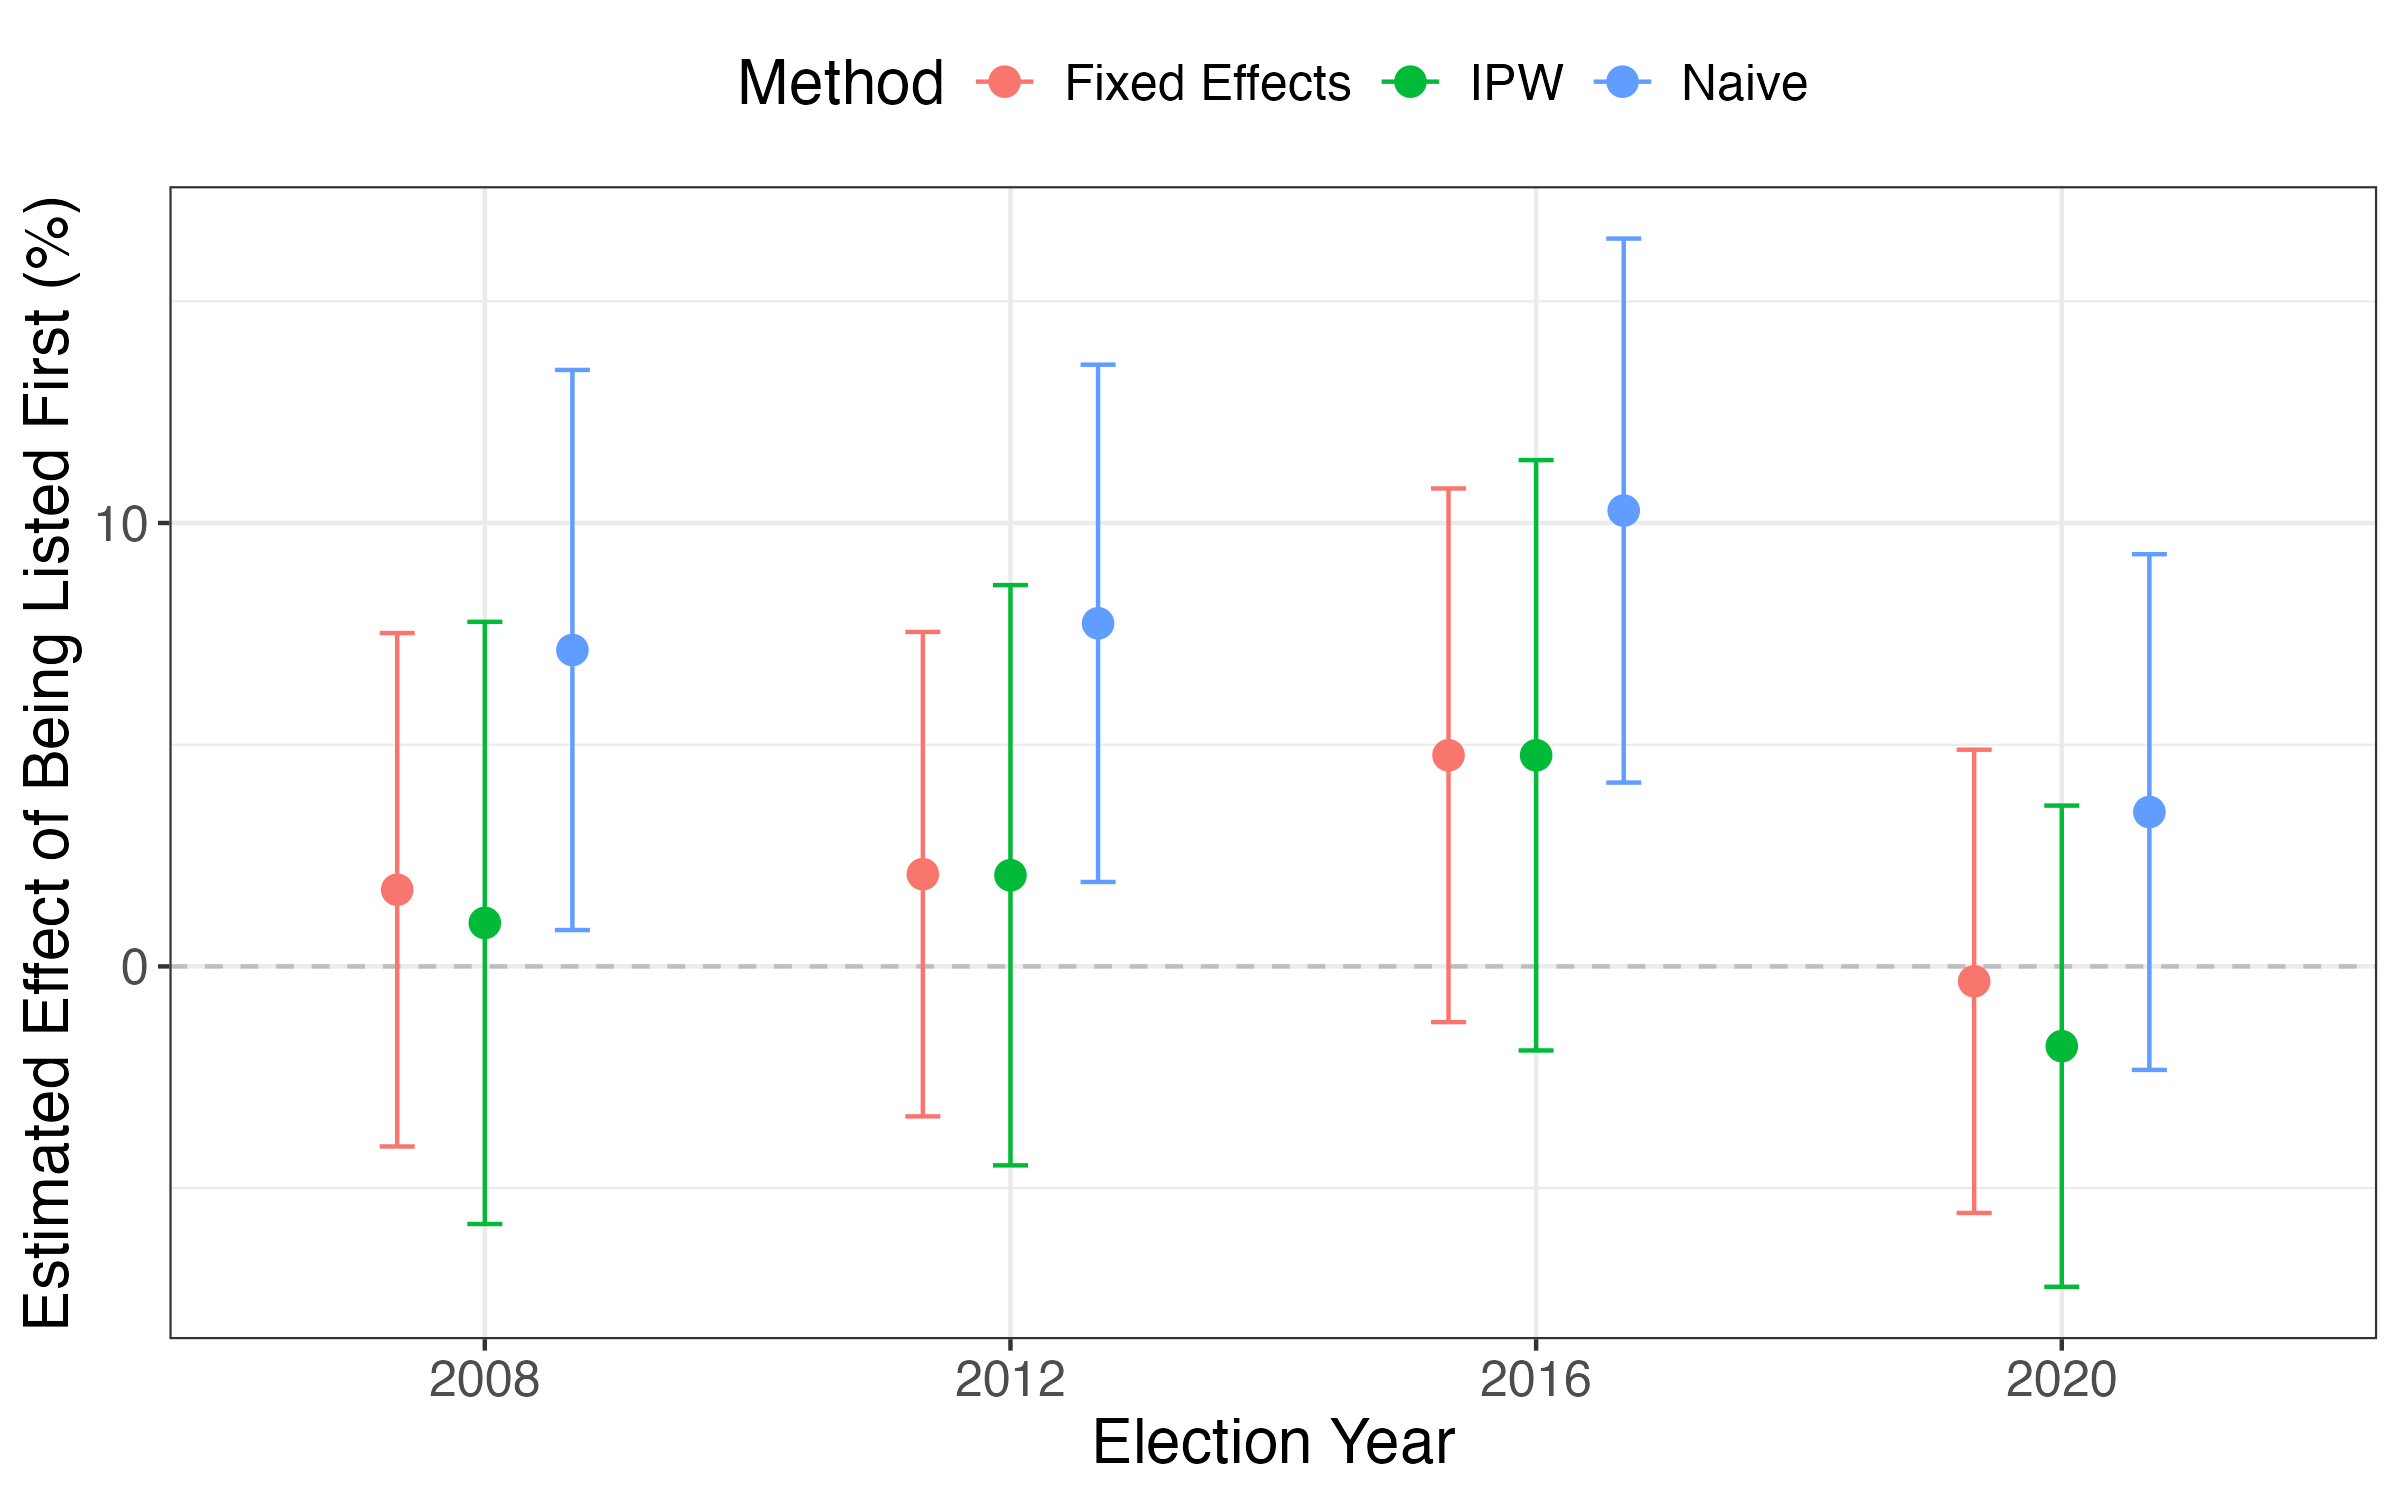
\includegraphics[width=0.7\textwidth]{../outputs/figures/effect_plot.png}
  \caption{Estimated Ballot Order Effect by Election Year and Method.}
  \caption*{\textit{Notes:} 
    The plot displays point estimates and 95\% confidence intervals 
    for the ballot order effect on vote share (\%)
    using three different methods: 
    naive comparison (blue), 
    \gls{fe} regression (red),
    and \gls{ipw} regression (green).
    All standard errors are calculated 
    using the HC2 variant of the \gls{ehw} sandard errors.}
  \label{fig:effect-plot}
\end{figure}

\subsection{Fisher Randomization Test Results}

\cref{tab:randomization-results} presents
the \gls{frt} results,
including the observed test statistics,
$p$-values,
and standard errors of the $p$-value estimates.
The results are valid regardless of potential interference,
as the \gls{frt} does not require \gls{sutva}.
For all four election years,
the null hypothesis of no ballot order effect
cannot be rejected at the conventional 0.05 significance level.

% This file is auto-generated by code/05_generate_latex_tables.R
 % Do not edit manually
 % Results from Fisher's exact randomization test
 % P-values computed via Monte Carlo with 10000 permutations
 % 
 % Required LaTeX packages:
 % \usepackage{booktabs}
 % \usepackage{threeparttable}
 % \usepackage{array}

\begin{table}[!h]
\centering
\caption{\label{tab:randomization-results}Randomization Inference Results for Ballot Order Effects.}
\centering
\begin{threeparttable}
\begin{tabular}[t]{lrrrr}
\toprule
Year & Test Statistic & P-value & P-value SE & Num. of Permutations\\
\midrule
2008 & $1.7288$ & $0.629$ & $0.005$ & 10000\\
2012 & $2.0801$ & $0.535$ & $0.005$ & 10000\\
2016 & $4.7613$ & $0.150$ & $0.004$ & 10000\\
2020 & $-0.3366$ & $0.910$ & $0.003$ & 10000\\
\bottomrule
\end{tabular}
\begin{tablenotes}[para]
\item \textit{Notes:} 
\item P-values computed via randomization inference with 10000 Monte Carlo permutations. *** $p < 0.001$, ** $p < 0.01$, * $p < 0.05$. Test statistic is the variance-weighted difference in means.
\end{tablenotes}
\end{threeparttable}
\end{table}

\cref{fig:randomization-distribution} displays
the randomization distributions
of the test statistic
for each election year.
Each panel shows the null distribution
of the weighted difference-in-means statistic,
with the observed statistic indicated by a vertical red line.
The $p$-value represents the proportion
of simulated statistics
at least as extreme as the observed value.
In all years,
the observed statistics fall well within
the null distribution,
resulting in large $p$-values
and failure to reject the null hypothesis.

\begin{figure}[htbp]
  \centering
  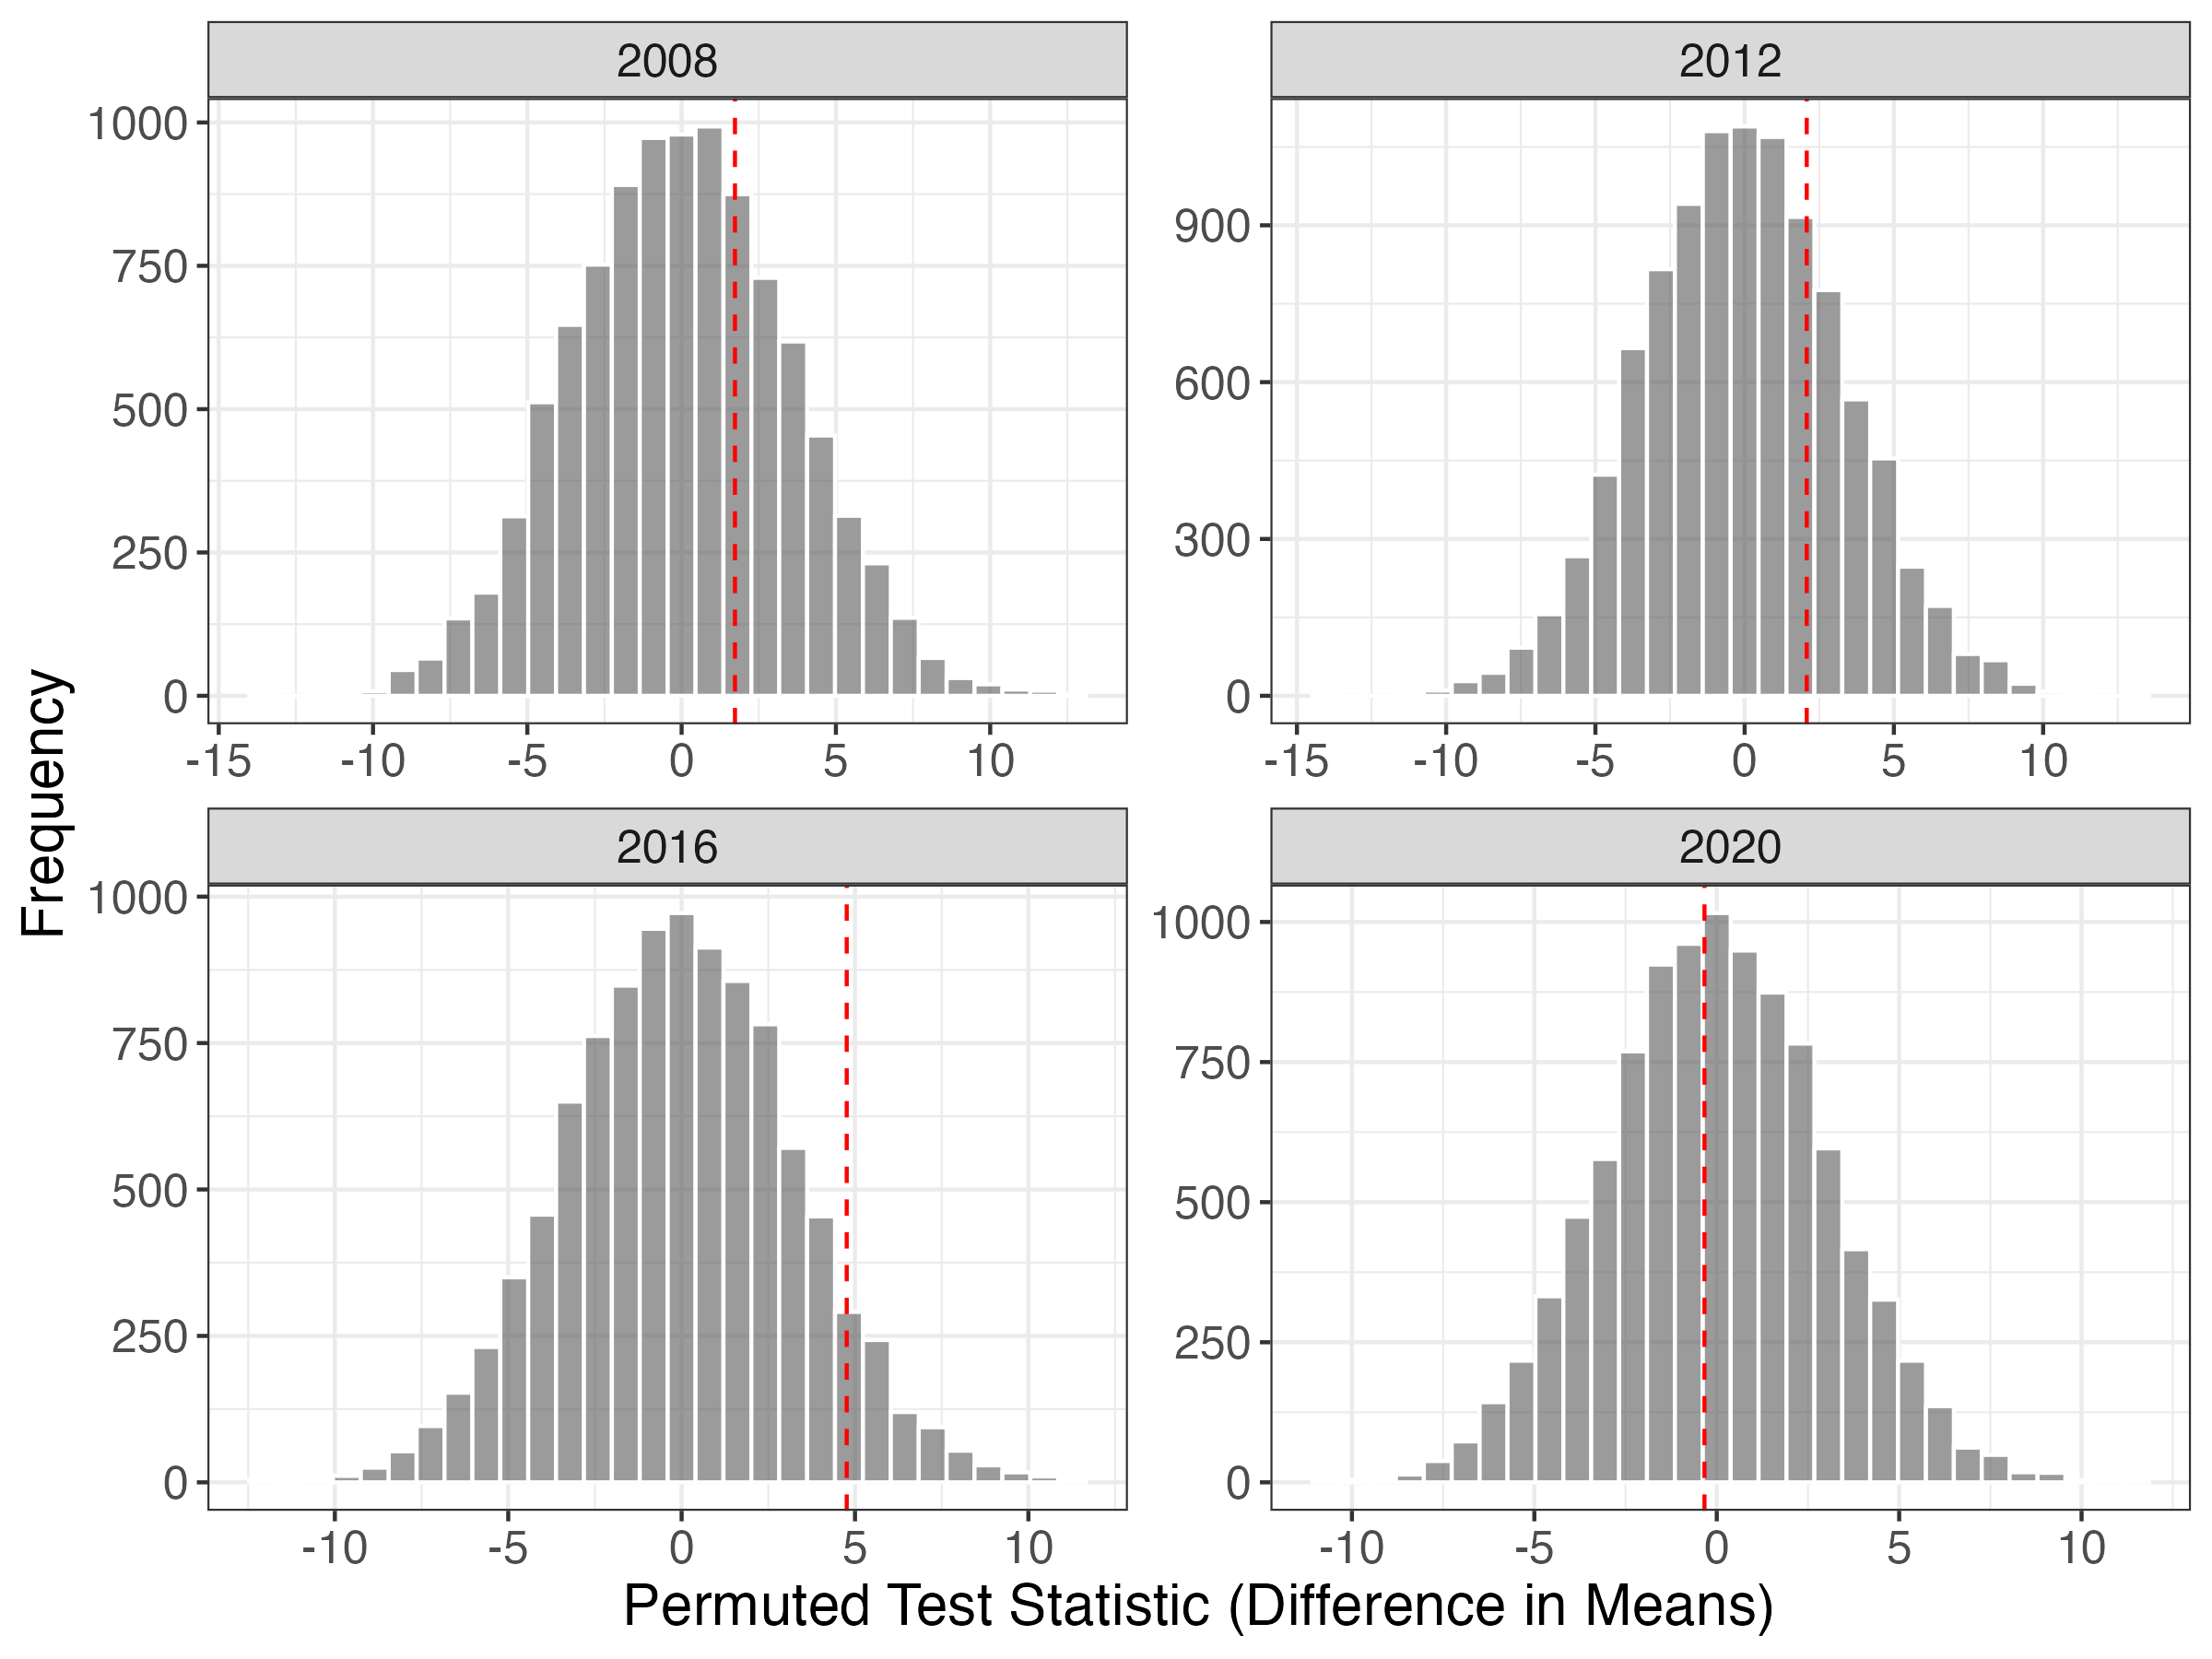
\includegraphics[width=0.8\textwidth]{../outputs/figures/randomization_distribution_diff_in_means_varw_plot.png}
  \caption{Randomization Distributions of the Test Statistic by Election Year.}
  \caption*{\textit{Notes:} 
    The vertical red line indicates the observed test statistic. 
  }
  \label{fig:randomization-distribution}
\end{figure}

\bibliographystyle{apalike}
\bibliography{../references}
\end{document}

